\documentclass[9pt]{beamer} 

% 
%==> Preamble
%
%
%==> Standard packages
%
\usepackage{hyperref, amsmath, amssymb, mathtools, hyperref, mathrsfs, enumerate}

%
%==> Graphics support
%
\usepackage{tikz}
\usetikzlibrary{backgrounds}
\usetikzlibrary{decorations.fractals}

%
%==> Custom commands
\newcommand{\w}{\omega}
\newcommand{\ow}{\overline{\omega}}

%
%==> Theme support
%
\usepackage{helvet}
\definecolor{links}{HTML}{2A1B81}
\hypersetup{colorlinks,linkcolor=,urlcolor=links}
\mode<presentation>{
	\usetheme{Pittsburgh}
	\usecolortheme{seagull}
	}
% Set all frame titles to bold faec
\setbeamerfont{frametitle}{series=\bfseries}
% Set default section counter to 0
%\setcounter{section}{-1}

%
%==> Code support
%
\usepackage{xcolor}
\usepackage{textcomp}
\usepackage{listings,algorithm,algorithmic}
\colorlet{verylightgray}{lightgray!10}

%
%==> LaTeX syntax highlighting + custom tikz library keywords
%
\lstset{
        language={[LaTeX]TeX},
        basicstyle=\ttfamily,
        texcsstyle={*\color{purple}\bfseries},
        keywordstyle=[1]\color{blue},
        keywordstyle=[2]\color{violet}, % Different colors for external functions
        moretexcs={draw, node, filldraw, foreach, x, usetikzlibrary},
        morekeywords={tikzpicture, tikz, backgrounds, decorations, fractals, grid, plot, at, to, circle, rectangle, arc, domain}, % External packages
        keywords=[2]{factorial, sqrt, pow, exp, ln, background, log10, log2, mod, floor, round, abs, ceil, sin, cos, tan, min, max, e, pi},
        backgroundcolor=\color{verylightgray},
        commentstyle=\color{gray},
        mathescape=false
}


%
%==> Begin document
%
\begin{document}

%
%==> Title page
%
%
%==> Title
%

\title{
  \bf A crash course on using Ti{\it k}Z
}

%
%==> Author
%
\author{
  Ben Cot\'e \& Jon Lo Kim Lin \\
  \href{mailto:cote@math.ucsb.edu}{\tt cote@math.ucsb.edu}\\
  \href{mailto:jlokimlin@math.ucsb.edu}{\tt jlokimlin@math.ucsb.edu}
}

%
%==> Date
%
\date{
  UCSB Hypatian Seminar\\
  04/21/14
}

\begin{frame}
  \maketitle
\end{frame}


%
%==> Outline
%
\begin{frame}
  \frametitle{Outline}
  \tableofcontents
\end{frame}

%
%==> Section 1: What is Tikz?
%
%
%==> Section 1: What is TikZ?
%
\section{
  What is Ti$k$Z?
}

%
%==> What is TikZ
%
\begin{frame}
  \frametitle{
    What is Ti$k$Z?
  }
  \begin{enumerate}
  \item
    A recursive acronym for \textcolor{blue}{ \tt Ti$k$Z ist kein Zeichenprogramm} (German for ``Ti$k$Z is not a drawing program").
  \item
    More specifically, Ti$k$Z is a package for creating pictures.
  \item
    Create anything from rectangles, circles to Koch snowflakes, 3D graphs and animations.
  \item
    Ti$k$Z works very well with Beamer (they were written by the same person!). Muck thanks and gratitude to Till Tantau.
  \end{enumerate}

\end{frame}

%
%==> An image by Ben Cot\'e
%
\begin{frame} 
  \frametitle{
    An image by Ben Cot\'e
}
  
  {
    \tiny
    \begin{center}
      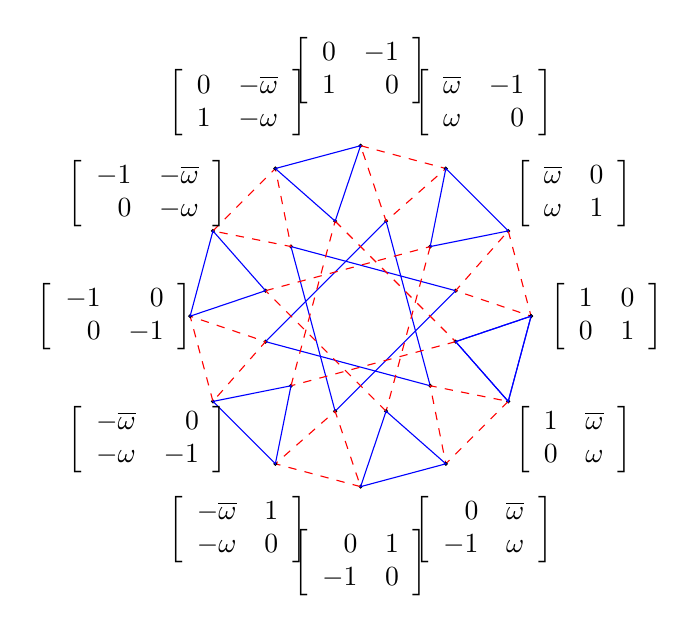
\begin{tikzpicture}[scale=1.25]
  \foreach \x in {15,75,...,330} {
    \filldraw[black] (\x:1cm) circle(0.4pt); % dots at each point
    % lines across inside
    \draw[blue] (\x:1cm) -- (\x-120:1cm);
  }
  \foreach \x in {45,105,...,345} {
    \filldraw[black] (\x:1cm) circle(0.4pt); % dots at each point
    % lines across outside
    \draw[red,dashed] (\x:1cm) -- (\x-120:1cm);
  }
  \foreach \x in {30,90,...,330} {
    \filldraw[black] (\x:1.73205cm) circle(0.4pt); % dots at each point
    % lines across inside
    \draw[red,dashed] (\x:1.73205cm) -- (\x-30:1.73205cm) -- (\x-15:1cm) -- cycle;
  }
  \foreach \x in  {0,60,...,360} {
    \filldraw[black] (\x:1.73205cm) circle(0.4pt); % dots at each point
    % lines across inside
    \draw[blue] (\x:1.73205cm) -- (\x-30:1.73205cm) -- (\x-15:1cm) -- cycle;
  }
  \foreach \x/\a/\b/\c/\d in {
    0/1/0/0/1,
    30/\ow/0/\w/1,
    60/\ow/-1/\w/0,
    90/0/-1/1/0,
    120/0/-\ow/1/-\w,
    150/-1/-\ow/0/-\w,
    180/-1/0/0/-1,
    210/-\ow/0/-\w/-1,
    240/-\ow/1/-\w/0,
    270/0/1/-1/0,
    300/0/\ow/-1/\w,
    330/1/\ow/0/\w
  }
  \draw (\x:2.5cm) node { $\left[ \begin{array}{rr} \a & \b \\  \c & \d \end{array}\right]$};      
\end{tikzpicture} 

    \end{center}
  }
  

\end{frame}

%
%==> Ben Cot\'e's source code
%
\begin{frame}[fragile]
  \frametitle{
    Ben Cot\'e's source code
  }

  {
    \tiny
    \lstinputlisting{./tex/src/image_by_ben.tex}
  }
  
\end{frame}

%
%==> Preliminaries
%
\begin{frame}[fragile]
  \frametitle{
    Preliminaries
  }

  \begin{enumerate}
  \item
    You need to add

    \begin{lstlisting}
      \usepackage{tikz}
    \end{lstlisting}

    to your document preamble. Other commands to put in preamble will be discussed later.
  \item
    When creating a picture use the {\tt tikzpicture} environment. E.g.

  \begin{lstlisting}
    \begin{tikzpicture}
      %
      %... code
      %
    \end{tikzpicture}
  \end{lstlisting}
  \end{enumerate}

\end{frame}


%
%==> Section 2: Drawing lines and curves
%
%
%==> Section: Drawing lines and curves
%
\section{
  Drawing lines and curves
}
%
%==> simple straight lines
%
\begin{frame}[fragile]
  \frametitle{
    Simples straight lines
  }
  To draw a line you do something like

  \lstinputlisting{./tex/src/draw_line.tex}
  
  and you get

  \begin{center}
    \begin{tikzpicture}
  \draw (0,0) --(1,2);
\end{tikzpicture}

  \end{center}
  
Ti$k$Z automatically draws a line between the points $(0,0)$ and $(1,2)$ and sets up the right space for the figure (by default, coordinates are in centimeters).
\end{frame}

%
%==> Sequence of segments
%
\begin{frame}

  You can do a sequence of segments which goes from point to point:

  \lstinputlisting{./tex/src/sequence_of_segments.tex}

  to get

  \begin{center}
    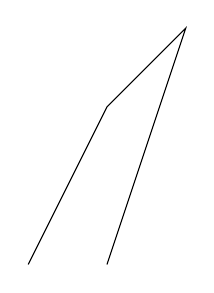
\begin{tikzpicture}
  \draw (0,0) --(1,2) -- (2,3) -- (1,0);
\end{tikzpicture}

  \end{center}
  
\end{frame}

%
%==> Add grid lines
%
\begin{frame}[fragile]

  We now have added the grid lines on the graphic to make it clearer. This is done through the command

  \begin{lstlisting}
    \draw[help lines] (0,0) grid (2,3);
  \end{lstlisting}

  which draws a grid from $(0,0)$ to $(2,3).$
  
  \lstinputlisting{./tex/src/add_grid_lines.tex}

  to get

  \begin{center}
    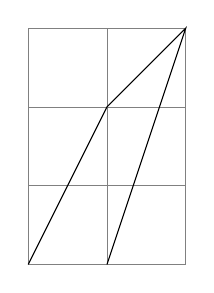
\begin{tikzpicture}
\draw[help lines] (0,0) grid (2,3);
\draw (0,0) --(1,2) -- (2,3) -- (1,0);
\end{tikzpicture}

  \end{center}

\end{frame}

%
%==> Add several lines
%
\begin{frame}[fragile]

  Of course, you can put several lines on the same graph:

  \lstinputlisting{./tex/src/add_several_lines.tex}

  yields

  \begin{center}
    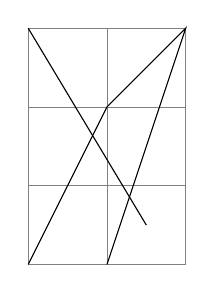
\begin{tikzpicture}
  \draw [help lines] (0,0) grid (2,3);
  \draw (0,0) --(1,2) -- (2,3) -- (1,0);
  \draw (0,3) -- (1.5,0.5);
\end{tikzpicture}

  \end{center}
  
  Notice the semi-colons ``; "at the end of lines -- they mark the end of instructions. That is, in the last picture we could have written

  {
    \footnotesize
    \begin{lstlisting}
      \draw (0,0) --(1,2) -- (2,3) -- (1,0); \draw (0,3) -- (1.5,0.5);
    \end{lstlisting}
  }
  
  without changing the output. You can also add and suppress spaces, for instance in order to make the code easier to read, without changing anything in the output.

\end{frame}

%
%==> Scaling pictures
%
\begin{frame}[fragile]
  \frametitle{
    Scaling pictures
  }

  One very useful feature of Ti$k$Z is that you can blow up the picture, by adding an option ``scale" to the environment.

  \begin{columns}
    \begin{column}{0.6\textwidth}
      \lstinputlisting{./tex/src/scaled_line.tex}
    \end{column}
    \begin{column}{0.4\textwidth}
      \begin{tikzpicture}[scale=2]
  \draw (0,0) -- (1,1);
\end{tikzpicture}

    \end{column}
  \end{columns}

  which you can compare to the following: 

  
  \begin{columns}
    \begin{column}{0.6\textwidth}
      \lstinputlisting{./tex/src/original_line.tex}
    \end{column}
    \begin{column}{0.4\textwidth}
      \begin{tikzpicture}
  \draw (0,0) -- (1,1);
\end{tikzpicture}

    \end{column}
  \end{columns}
  
\end{frame}
% Scaling in one dimension
\begin{frame}[containsverbatim]
You can scale only one dimension:

  \begin{columns}
    \begin{column}{0.6\textwidth}
      \lstinputlisting{./tex/src/scale_one_dimension.tex}
    \end{column}
    \begin{column}{0.4\textwidth}
      \begin{tikzpicture}[xscale=3]
  \draw (0,0) -- (1,1);
\end{tikzpicture}

    \end{column}
  \end{columns}


or both dimensions in different proportions:

  \begin{columns}
    \begin{column}{0.6\textwidth}
      \lstinputlisting{./tex/src/scale_both_dimensions.tex}
    \end{column}
    \begin{column}{0.4\textwidth}
      \begin{tikzpicture}[xscale=2.5,yscale=0.5]
  \draw (0,0) -- (1,1);
\end{tikzpicture}

    \end{column}
  \end{columns}

\end{frame}

%
%==> Arrows and the like
%
\begin{frame}[fragile]
  \frametitle{
    Arrows and the like
  }

  You can ``decorate" the lines. For instance we can put arrows or bars on one of both extremities:

  \lstinputlisting{./tex/src/decorate_lines.tex}
  
  which yields

  \begin{center}
    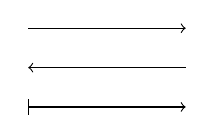
\begin{tikzpicture}
  \draw [->] (0,0) -- (2,0);
  \draw [<-] (0, -0.5) -- (2,-0.5);
  \draw [|->] (0,-1) -- (2,-1);
\end{tikzpicture}

  \end{center}
  
\end{frame}
%
%==> Coordinates
%
\begin{frame}[fragile]

  When you draw several segments, the arrows are placed at the extremities of the first and the last segments. This is convenient, among other things to draw axes (we will see later how to label them):

  \lstinputlisting{./tex/src/coordinates.tex}
  
which gives you

  \begin{center}
    \begin{tikzpicture}
  \draw [<->] (0,2) -- (0,0) -- (3,0);
\end{tikzpicture}

  \end{center}
  
\end{frame}
%
%==> Changing the thickness of lines
%
\begin{frame}[fragile]
  \frametitle{
    Changing the thickness of lines
  }

  Other decorations include changing the thickness:

  \lstinputlisting{./tex/src/change_line_thickness.tex}
  
  which gives you

  \begin{center}
    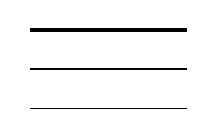
\begin{tikzpicture}
  \draw [ultra thick] (0,1) -- (2,1);
  \draw [thick] (0,0.5) -- (2,0.5);
  \draw [thin] (0,0) -- (2,0);
\end{tikzpicture}

  \end{center}
  
\end{frame}
%
%==> helplines
%
\begin{frame}[fragile]
  \frametitle{
    The help lines option
  }

  There is also the {\tt help lines} option, discussed earlier, which is made specially to be fine gray lines for showing special points:

    \lstinputlisting{./tex/src/add_help_lines.tex}
  
  which yields.

  \begin{center}
    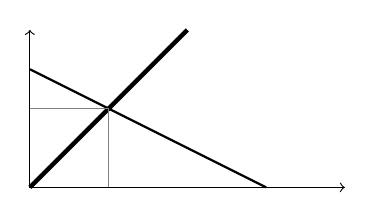
\begin{tikzpicture}
  \draw [<->] (0,2) -- (0,0) -- (4,0);
  \draw [thick] (0,1.5) -- (3,0);
  \draw [ultra thick] (0,0) -- (2,2);
  \draw [help lines] (1,0) -- (1,1) -- (0,1);
\end{tikzpicture}

  \end{center}
  
\end{frame}
%
%==> Custom line widths
%
\begin{frame}[fragile]
  \frametitle{
    Custom line widths
  }

  You can also use custom widths:

  \lstinputlisting{./tex/src/custom_line_widths.tex}
  
  which gives a line 12pt wide (the default dimension for width is point) and another one .2cm wide:

  \begin{center}
    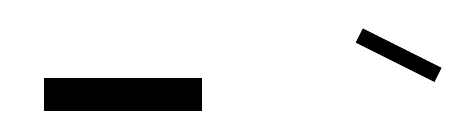
\begin{tikzpicture}
  \draw [line width=12] (0,0) -- (2,0);
  \draw [line width=0.2cm] (4,.75) -- (5,.25);
\end{tikzpicture}

  \end{center}
  
\end{frame}
%
%==> Dashes and dots
%
\begin{frame}[fragile]
  \frametitle{
    Dashes and dots
  }

  You can also make dashed and dotted lines

  \lstinputlisting{./tex/src/dashes_and_dots.tex}

  This gives:

    \begin{center}
    \begin{tikzpicture}
  \draw [dashed, ultra thick] (0,1) -- (5,1);
  \draw [dashed] (0, 0.5) -- (5,0.5);
  \draw [dotted] (0,0) -- (5,0);
\end{tikzpicture}

    \end{center}

    The top line shows you that you can mix types of decorations. You have lots of control over the style of your dotted and dashed lines (see the manual).

\end{frame}
%
%==> Colored lines
%
\begin{frame}[fragile]
  \frametitle{
    Colored lines
  }

  And finally, you can color your lines.

  \lstinputlisting{./tex/src/colored_lines.tex}

   We obtain

    \begin{center}
    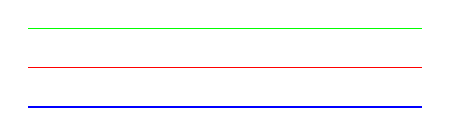
\begin{tikzpicture}
  \draw [green] (0,1) -- (5,1);
  \draw [red] (0, 0.5) -- (5,0.5);
  \draw [blue] (0,0) -- (5,0);
\end{tikzpicture}

    \end{center}

\end{frame}

%
%==> Taste the rainbow
%
\begin{frame}
  \frametitle{
    Taste the rainbow
  }
  You have direct access to the following pre-defined colors: red 
\begin{tikzpicture} \draw [red, line width=6]
     (0,0) -- (.5,0);  \end{tikzpicture}, 
green 
\begin{tikzpicture} \draw [green, line width=6]
     (0,0) -- (.5,0);  \end{tikzpicture}, blue 
\begin{tikzpicture} \draw [blue, line width=6]
     (0,0) -- (.5,0);  \end{tikzpicture}, cyan 
\begin{tikzpicture} \draw [cyan, line width=6]
     (0,0) -- (.5,0);  \end{tikzpicture}, magenta 
\begin{tikzpicture} \draw [magenta, line width=6]
     (0,0) -- (.5,0);  \end{tikzpicture}, yellow 
\begin{tikzpicture} \draw [yellow, line width=6]
     (0,0) -- (.5,0);  \end{tikzpicture}, black 
\begin{tikzpicture} \draw [black, line width=6]
     (0,0) -- (.5,0);  \end{tikzpicture}, darkgray\footnote{An affront to the King's language} 
\begin{tikzpicture} \draw [darkgray, line width=6]
     (0,0) -- (.5,0);  \end{tikzpicture}, light gray 
\begin{tikzpicture} \draw [lightgray, line width=6]
     (0,0) -- (.5,0);  \end{tikzpicture}, brown 
\begin{tikzpicture} \draw [brown, line width=6]
     (0,0) -- (.5,0);  \end{tikzpicture}, lime 
\begin{tikzpicture} \draw [lime, line width=6]
     (0,0) -- (.5,0);  \end{tikzpicture}, olive 
\begin{tikzpicture} \draw [olive, line width=6]
     (0,0) -- (.5,0);  \end{tikzpicture}, orange 
\begin{tikzpicture} \draw [orange, line width=6]
     (0,0) -- (.5,0);  \end{tikzpicture}, pink 
\begin{tikzpicture} \draw [pink, line width=6]
     (0,0) -- (.5,0);  \end{tikzpicture}, purple 
\begin{tikzpicture} \draw [purple, line width=6]
     (0,0) -- (.5,0);  \end{tikzpicture}, teal 
\begin{tikzpicture} \draw [teal, line width=6]
     (0,0) -- (.5,0);  \end{tikzpicture}, violet 
\begin{tikzpicture} \draw [violet, line width=6]
     (0,0) -- (.5,0);  \end{tikzpicture}, and white \begin{tikzpicture} \draw [white, line width=6]
  (0,0) -- (.5,0);  \end{tikzpicture}. And you can define all the colors you might want using the RGB color model (see the manual).
\end{frame}

%
%==> Pictures in the middle of text
%
\begin{frame}[fragile]
  \frametitle{
    Pictures in the middle of text
  }

  By the way, you may wonder how we included these rectangles in the text. Ti$k$Z makes a picture wherever 
\begin{tikzpicture}
  \draw [blue, line width=6] (0,0) -- (.5,0);
\end{tikzpicture}
 you want; we just typed

  \begin{center}
    \lstinputlisting{./tex/src/blue_in_middle_of_text.tex}
  \end{center}

  wherever we want in the text. To make these constructions easier to type you can use the command {\tt \bf \textbackslash tikz}  (see the manual).

\end{frame}

%
%==> Curves
%
\begin{frame}[fragile]
  \frametitle{
    Curves
  }

  We are not limited to straight lines:

  { \footnotesize
  \lstinputlisting{./tex/src/shapes.tex}
  }
  
  This gives:

  \begin{center}
    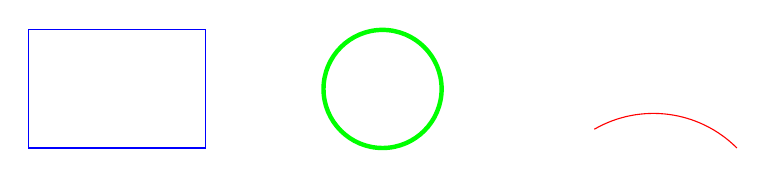
\begin{tikzpicture}[scale=1.5]
  \draw [blue] (0,0) rectangle (1.5,1);
  \draw [green, ultra thick] (3,0.5) circle [radius=0.5];
  \draw [red] (6,0) arc [radius=1, start angle=45, end angle= 120];
\end{tikzpicture}

  \end{center}

  The arc is of radius 1, starts at the point $(6,0)$ leaving it at an angle of $45^\circ$ and stops when its slope is $120^\circ$.

\end{frame}

%
%==> Smoother curves
%
\begin{frame}[fragile]
  \frametitle{
    Smoother curves
  }

  We can make paths take smoother turns:

  { \footnotesize
  \lstinputlisting{./tex/src/rounded_corners.tex}
  }
  
  which gives us

  \begin{center}
    \begin{tikzpicture}
  \draw [<->, rounded corners, thick, purple] (0,2) -- (0,0) -- (3,0);
\end{tikzpicture}

  \end{center}

\end{frame}
%
%==> Hard coding graphs
%
\begin{frame}[containsverbatim]
  \frametitle{
    Hard coding graphs
  }

  If you want a precise curve you can do it by computing lots of points in a program such as C/C++, Fortran, Python, MATLAB, etc, and then putting them into Ti$k$Z: 

  {
    \scriptsize
    \lstinputlisting{./tex/src/hard_coded_graph.tex}
  }
  
\end{frame}

%
%==> Hard coded graph results
%
\begin{frame}[containsverbatim]
    \frametitle{
    Hard coded graph results
    }

    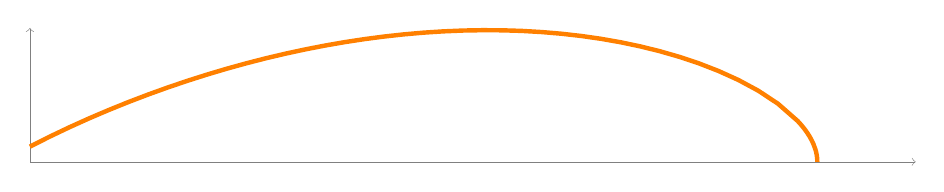
\begin{tikzpicture}[xscale=25,yscale=5]
  \draw [<->, help lines] (0.6,1.34) -- (0.6,1) -- (1.05,1);
  \draw [orange, ultra thick] (0.6, 1.0385) --
(0.61, 1.06372) -- (0.62, 1.08756) -- (0.63, 1.11012) -- (0.64,
1.13147) -- (0.65, 1.15166) -- (0.66, 1.17074) -- (0.67, 1.18874) -- (0.68,
1.20568) -- (0.69, 1.22157) -- (0.7, 1.23643) -- (0.71, 1.25026) -- (0.72,
1.26307) -- (0.73, 1.27486) -- (0.74, 1.28561) -- (0.75, 1.29534) -- (0.76,
1.30402) -- (0.77, 1.31165) -- (0.78, 1.31821) -- (0.79, 1.32369) -- (0.8,
1.32806) -- (0.81, 1.33131) -- (0.82, 1.3334) -- (0.83, 1.33431) -- (0.84,
1.334) -- (0.85, 1.33244) -- (0.86, 1.32956) -- (0.87, 1.32533) -- (0.88,
1.31966) -- (0.89, 1.3125) -- (0.9, 1.30373) -- (0.91, 1.29325) -- (0.92,
1.2809) -- (0.93, 1.26649) -- (0.94, 1.24976) -- (0.95, 1.23032) -- (0.96,
1.2076) -- (0.97, 1.18065) -- (0.98, 1.14763) -- (0.99, 1.1038) -- (0.991,
1.09836) -- (0.992, 1.09261) -- (0.993, 1.0865) -- (0.994, 1.07994) -- (0.995,
1.07282) -- (0.996, 1.06497) -- (0.997, 1.0561) -- (0.998, 1.04563) -- (0.999,
1.03209) -- (0.9991, 1.03042) -- (0.9992, 1.02866) -- (0.9993,
1.02679) -- (0.9994, 1.02478) -- (0.9995, 1.0226) -- (0.9996, 1.02019) -- (0.9997,
1.01747) -- (0.9998, 1.01424) -- (0.9999, 1.01005) -- (0.9999,
1.01005) -- (0.99991, 1.00953) -- (0.99992, 1.00898) -- (0.99993,
1.0084) -- (0.99994, 1.00778) -- (0.99995, 1.0071) -- (0.99996,
1.00634) -- (0.99997, 1.00549) -- (0.99998, 1.00448) -- (0.99999, 1.00317) -- (1,1);
\end{tikzpicture}


    \begin{enumerate}
    \item
      This was overkill: We do not need so many points;
    \item
      This can also serve as a reminder that one Ti$k$Z instruction can be spread over several lines and cut arbitrarily over several lines. The marker is the semi-colon, not the end of line!
    \end{enumerate}

\end{frame}

%
%==> Plot curve
%
\begin{frame}[fragile]

  There are a number of ways by which you can do curves without plotting all the points. Here is an easy one:

  \lstinputlisting{./tex/src/plot_curve.tex}
  
  This gives us a curve from $(0,0)$ to $(2,1.5)$ which leaves at an angle of $90^\circ$ and arrive at an angle of $195^\circ$: Notice that we replaced the \textcolor{red}{\tt  --} with \textcolor{red}{\tt to}.

  \begin{center}
    \begin{tikzpicture}[scale=3]
  \draw [very thick] (0,0) to [out=90,in=195] (2,1.5);
\end{tikzpicture}

  \end{center}
  
\end{frame}
%
%==> Replacing -- with to
%
\begin{frame}
  \frametitle{
    Replacing \textbf{\tt  --} with \textbf{\tt to}
  }

  \begin{center}
    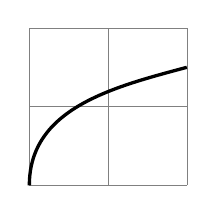
\begin{tikzpicture}
      \draw [style=help lines] (0,0) grid (2,2);
      \draw [very thick] (0,0) to [out=90,in=195] (2,1.5);
    \end{tikzpicture}
  \end{center}
  
  \begin{enumerate}
  \item
    When the curves goes \textcolor{red}{out} of $(0,0),$ you put a needle with one extremity on the starting point and the other one facing right and you turn it counterclockwise until it is tangent to the curve. The angle by which you have to turn the needle gives you the \textcolor{red}{out} angle.
  \item
    When the curves goes \textcolor{red}{in} at $(2,1.5),$ you put a needle with one extremity on the arrival point and the other one facing right and you turn it counterclockwise until it is tangent to the curve. The angle by which you have to turn the needle gives you the \textcolor{red}{in} angle.
  \end{enumerate}

\end{frame}

%
%==> Several to instructions
%
\begin{frame}[fragile]
  \frametitle{
    Several \textbf{\tt to} instructions
  }
  
  As with straight lines you can put several \textbf{\tt to} instructions in the same Ti$k$Z instruction:

  \lstinputlisting{./tex/src/several_to_instructions.tex}
  
  we obtain:

  \begin{center}
    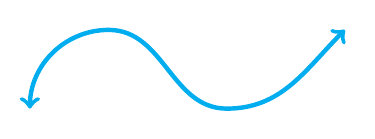
\begin{tikzpicture}
  \draw [<->,ultra thick, cyan]
  (0,0) to [out=90,in=180]
  (1,1) to [out=0,in=180]
  (2.5,0) to [out=0,in=-135] (4,1);
\end{tikzpicture}

  \end{center}
  
\end{frame}


%
%==> Section 3: Plotting functions
%
%
%==> Section: Plotting functions
%
\section{
  Plotting functions
}
%
%==> Plotting user-defined functions
%
\begin{frame}[fragile]
  \frametitle{
    Plotting user-defined functions
  }

  Ti$k$Z also has a math engine which enables you to plot functions:

  \lstinputlisting{./tex/src/plot_function.tex}

  gives you

  \begin{center}
    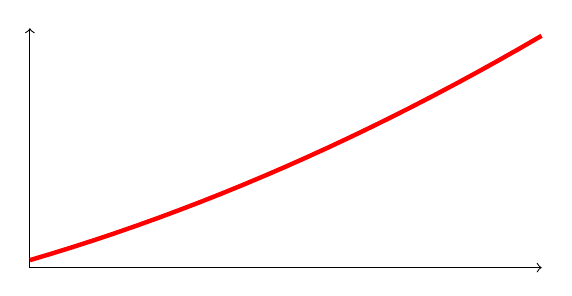
\begin{tikzpicture}[xscale=13,yscale=3.8]
  \draw [<->] (0,0.8) -- (0,0) -- (0.5,0);
  \draw[red, ultra thick, domain=0:0.5]
  plot (\x, {0.025+\x+\x*\x});
\end{tikzpicture}

  \end{center}

  The domain instruction shows the range of $x$ which is plotted. In this case we are plotting the function $0.025+x+x^2.$ Note the braces around the function that we plot in

  \begin{lstlisting}
    plot (\x, {function});
  \end{lstlisting}
  
\end{frame}

%
%==> Built-in math functions
%
\begin{frame}[fragile]
  \frametitle{
    Built-in math functions
}

  \begin{itemize}
  \item
    Many mathematical functions are possible; you will probably have enough with

    \begin{lstlisting}
      factorial(\x), sqrt(\x), exp(\x), ln(\x)
      log2(\x), log10(\x), abs(\x)
    \end{lstlisting}

  \item
    
    \begin{lstlisting}
      pow(\x,y), mod(\x, y)
    \end{lstlisting}

    which gives $x^y$ and $x$ modulo $y.$

  \item
    
    \begin{lstlisting}
      round(\x), floor(\x), ceil(\x)
    \end{lstlisting}
       
    rounds $x$ to the nearest integer, the largest integer smaller than $x$, the smallest integer larger than $x$.
  \end{itemize}
\end{frame}


%
%==> Built-in math functions (continued)
%
\begin{frame}[fragile]
  \frametitle{
    Built-in math functions (continued)
}

  \begin{itemize}
  \item
    \begin{lstlisting}
      sin(\x)
    \end{lstlisting}

    it assumes that $x$ is in degrees; if $x$ is expressed in radians use

    \begin{lstlisting}
      sin(\x r)
    \end{lstlisting}

    In a similar fashion,
    
    \begin{lstlisting}
      cos(\x), cos(\x r), tan(\x), tan(\x r)
    \end{lstlisting}

    We also have

    \begin{lstlisting}
      min(\x,y), max(\x,y).
    \end{lstlisting}
    
  \item 
    In mathematical expressions the two following \textcolor{violet}{\bf rational} variables can be useful:

    \begin{lstlisting}
      e
    \end{lstlisting}
    
    which is equal to \textcolor{violet}{2.718281828}, and

    \begin{lstlisting}
      pi
    \end{lstlisting}

    which is equal to \textcolor{violet}{3.141592654}.

  \end{itemize}
\end{frame}

%
%==> Plot trig functions
%
\begin{frame}[fragile]
  
  You can mix functions to compute more complicated expressions (see above for the reason for the {\tt r} parameter in the argument of $\sin$ and $\cos$ and note the use of \textcolor{violet}{\tt pi} to define the domains):
  \lstinputlisting{./tex/src/plot_trig_functions.tex}

  which gives you

  \begin{center}
    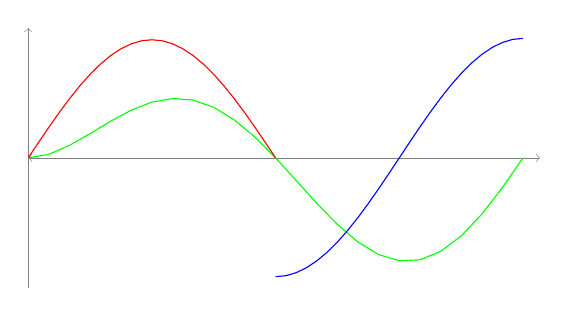
\begin{tikzpicture}[yscale=1.5]
  \draw [help lines, <->] (0,0) -- (6.5,0);
  \draw [help lines, ->] (0,-1.1) -- (0,1.1);
  \draw [green,domain=0:2*pi]
  plot (\x, {(sin(\x r)* ln(\x+1))/2});
  \draw [red,domain=0:pi]
  plot (\x, {sin(\x r)});
  \draw [blue, domain=pi:2*pi]
  plot (\x, {cos(\x r)*exp(\x/exp(2*pi))});
\end{tikzpicture}

  \end{center}

\end{frame}


%
%==> Section 4: Putting labels in pictures
%
%
%==> Section: Putting labels in pictures
%
\section{
  Putting labels in pictures
}

\begin{frame}[fragile]
  \frametitle{
    Putting labels in pictures
}

  When you construct a picture, in 99\% of cases you also need to put labels. This is easy! Let us start by seeing how we would place some text in a picture.

  \lstinputlisting{./tex/src/put_text_in_pictures.tex}
  
  yields

  \begin{center}
    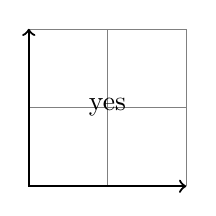
\begin{tikzpicture}
  \draw [help lines] (0,0) grid (2,2);
  \draw [thick, <->] (0,2) -- (0,0) -- (2,0);
  \node at (1,1) {yes};
\end{tikzpicture}

  \end{center}

 Notice how the ``yes" is positioned: the center of its ``baseline" is at $(1,1).$

\end{frame}

%
%==> Relative positioning 
%
\begin{frame}[fragile]
  \frametitle{
    Relative positioning
  }

  Sometimes you want a label to be situated relative to a point. Ti$k$Z has neat
  commands for this. For instance you can write

  \lstinputlisting{./tex/src/relative_positioning.tex}
  
  to get

  \begin{center}
    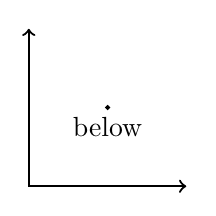
\begin{tikzpicture}
  \draw [thick, <->] (0,2) -- (0,0) -- (2,0);
  \draw[fill] (1,1) circle [radius=0.025];
  \node [below] at (1,1) {below};
\end{tikzpicture}

    \end{center}

\end{frame}

%
%==> More relative positioning
%
\begin{frame}[fragile]

  You are not limited to put things below a point:

  \lstinputlisting{./tex/src/more_relative_positioning.tex}
  
  yields
  
  \begin{center}
    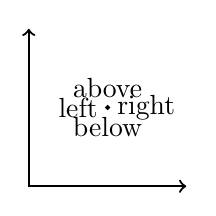
\begin{tikzpicture}
  \draw [thick, <->] (0,2) -- (0,0) -- (2,0);
  \draw [fill] (1,1) circle [radius=0.025];
  \node [below] at (1,1) {below};
  \node [above] at (1,1) {above};
  \node [left] at (1,1) {left};
  \node [right] at (1,1) {right};
\end{tikzpicture}

  \end{center}

\end{frame}
%
%==> Mix and match positioning
%
\begin{frame}[fragile]
  
  And, you can also mix and match

  \lstinputlisting{./tex/src/mix_and_match_positioning.tex}
  
  yields

  \begin{center}
    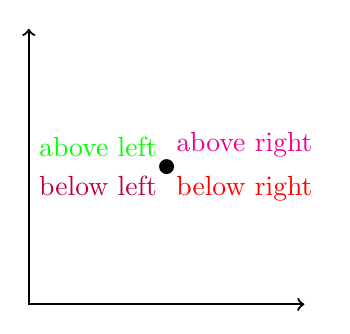
\begin{tikzpicture}[scale=3.5]
  \draw [thick, <->] (0,1) -- (0,0) -- (1,0);
  \draw[fill] (.5,.5) circle [radius=0.025];
  \node [below right, red] at (.5,.5) {below right};
  \node [above left, green] at (.5,.5) {above left};
  \node [below left, purple] at (.5,.5) {below left};
  \node [above right, magenta] at (.5,.5) {above right};
\end{tikzpicture}

  \end{center}

\end{frame}

%
%==> Labeling axes and points
%
\begin{frame}[fragile]
  \frametitle{
    Labeling axes and points
  }

  \lstinputlisting{./tex/src/label_axes_and_points.tex}
  
  gives us
  
  \begin{center}
    \begin{tikzpicture}[xscale=3, yscale=1.5]
  \draw [thick, <->] (0,1) -- (0,0) -- (1,0);
  \node [below right] at (1,0) {$x$};
  \node [left] at (0,1) {$y$};
  \draw [fill] (.4,.6) circle [radius=.5pt];
  \node[above right] (.4,.6) {$A$};
\end{tikzpicture}

  \end{center}

\end{frame}

%
%==> Supressing \node
%
\begin{frame}[fragile]

  You can avoid some typing by mixing nodes in the middle of paths. For instance the last figure could have been written as follows:

  \lstinputlisting{./tex/src/label_axes_and_points_alt.tex}
  
  which would have given exactly the same result. Note that the node is put after the point to which it is attached and that we suppress the $\backslash$ in

  \begin{lstlisting}
    \node
  \end{lstlisting}
  

\end{frame}

%
%==> Fancy nodes
%
\begin{frame}[containsverbatim]
  \frametitle{
    Fancy nodes
  }

  You may want to put several lines in your ``node" (this is convenient when drawing time lines for instance). This can be done by using the standard \LaTeX\, for indicating a new line but you must tell Ti$k$Z how to align things. From

  {
    \scriptsize
    \lstinputlisting{./tex/src/fancy_nodes.tex}
  }
  
  we obtain

  \begin{center}
    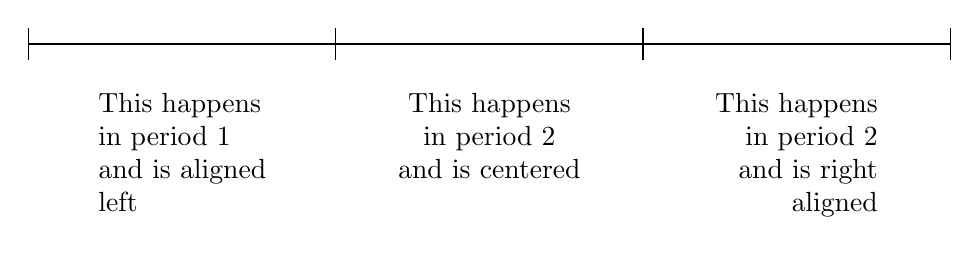
\begin{tikzpicture}[xscale=1.3]
  \draw [thick] (0,0) -- (9,0);
  \draw (0,-.2) -- (0, .2);
  \draw (3,-.2) -- (3, .2);
  \draw (6,-.2) -- (6, .2);
  \draw (9,-.2) -- (9, .2);
  \node[align=left, below] at (1.5,-.5)%
       {This happens\\in period 1\\and is aligned\\ left};
  \node[align=center, below] at (4.5,-.5)%
       {This happens\\in period 2\\and is centered};
  \node[align=right, below] at (7.5,-.5)%
       {This happens\\in period 2\\and is right\\aligned};
\end{tikzpicture}

  \end{center}
  
\end{frame}


%
%==> Section 5: TikZ libraries
%
%
%==> Section: TikZ libraries
%
\section{
  Ti$k$Z libraries
}
%
%==> TikZ libraries
%
\begin{frame}
  \frametitle{
    Ti$k$Z libraries
  }
  \begin{itemize}
  \item
    To provide simpler methods to create complex structures
    libraries for Ti$k$Z has \textcolor{purple}{\tt $\backslash$usetikzlibary}
  \item
    Different examples are: \textcolor{blue}{ \tt decorations.fractals},  \textcolor{blue}{ \tt arrows}, \textcolor{blue}{ \tt backgrounds}, \textcolor{blue}{ \tt intersections}, and \textcolor{blue}{ \tt shapes.geometric}.
  \end{itemize}
\end{frame}

%
%==> Examples
%
\begin{frame}[fragile]
  \frametitle{
    And now for some examples
  }

  First you must add

  \begin{lstlisting}
    \usetikzlibrary{backgrounds}
  \end{lstlisting}
  
  to your preamble

  \begin{center}
    \begin{tikzpicture}
  [background rectangle/.style={fill=blue!20,
      draw=blue!50,line width=3pt},
    show background rectangle]
  \draw[line width=2pt,color=gray]
  (2,2) circle[radius=1];
\end{tikzpicture}

  \end{center}

  \lstinputlisting{./tex/src/tikz_lib_backgrounds_example.tex}

\end{frame}

%
%==> Koch snowflake
%
\begin{frame}[fragile]
  \begin{itemize}
  \item
    For the Koch snowflake, first you must add

    \begin{lstlisting}
      \usetikzlibrary{decorations.fractals}
    \end{lstlisting}

    to your preamble

    % Generate image
    \begin{center}
      \begin{tikzpicture}[decoration=Koch
          snowflake,draw=blue,fill=green!20,thick]
        \filldraw decorate{ decorate{ (0,0) --
            ++(60:1) -- ++(-60:1) -- cycle}};
      \end{tikzpicture}
    \end{center}
    
    % Source file
    \begin{lstlisting}
      \begin{tikzpicture}[decoration=Koch
          snowflake,draw=blue,fill=green!20,thick]
        \filldraw decorate{ decorate{ (0,0) --
            ++(60:1) -- ++(-60:1) -- cycle}};
      \end{tikzpicture}
    \end{lstlisting}

  \item
    Don't forget to put the correct Ti$k$Z library in your preamble.
    
  \end{itemize}

\end{frame}


%
%==> Section 6: Conclusion
%
%
%==> Section: Conclusion
%
\section{
  Conclusion
}

%
%==> Conclusion
%
\begin{frame}
  \frametitle{
    Conclusion
  }

  \begin{enumerate}
  \item
    Ti$k$Z is an enormous program. You will find commands to draw hierarchical trees, to draw lots of different types of shapes, to do some elementary programming, to align elements of a picture in a matrix frame, to decorate nodes, to compute the intersections of paths, etc
  \item
     For a gentle introduction see: \href{http://cremeronline.com/LaTeX/minimaltikz.pdf}{A very minimal introduction to TikZ}.
  \item
    If you conundrum is not addressed in these slides it's probably somewhere in the exhaustive manual available at \href{http://paws.wcu.edu/tsfoguel/tikzpgfmanual.pdf}{tikzpgfmanual}
  \item
    Post questions on \href{http://tex.stackexchange.com/}{TeX - \LaTeX\ Stack Exchange}, a question and answer site for users of TeX, \LaTeX, ConTeXt, and related typesetting systems. It's 100\% free, no registration required. 
  \end{enumerate}
  
\end{frame}


%
%==> Thank you for your time
%
\begin{frame}

  \begin{center}
    {
      \huge \bf Thank you for your time
    }
  \end{center}

\end{frame}

%
%===> End document
%
\end{document}
